% !TEX root = ../convolutional_w2.tex

\begin{figure*}[t]\centering
% \myFigCol{street-11}{street-10}
% \myFigCol{green-2}{red-5}
%\myFigCol{green-6}{red-5}
% \myFigCol{street-2}{street-7}
% \myFigCol{street-8}{street-1}
\myFigCol{colors9}{street-11}
\vspace{-2mm}
\caption{
Color transfer with 2D convolutional transportation over the chrominance space.
Top row: evolution of the color-corrected image $f_1^\alpha$ as a function of $\alpha=(1-t,t)$.
Middle row: evolution of $f_2^\alpha$.
The red (resp. blue) framed image shows the input $f_1$ (resp.\ $f_2$) which is obtained for $t=0$ (resp.\ $t=1$).
Bottom row: barycenter histogram $\mu$ as a function of $t$; colors encode the corresponding position $x$ over the $(a,b)$ domain while luminance corresponds to the amplitude of $\mu(x)$ (zero being white).
}
\label{fig:ColorTransfer}
\vspace{-2mm}
\end{figure*}

\section{Discussion and Conclusion}
%\vspace{-2mm}
Although optimal transportation has long been an attractive potential technique for graphics applications, optimization challenges hampered efforts to include it as part of the standard toolbox.  Convolutional Wasserstein distances comprise a large step toward closing the gap between theory and practice.  They are easily computable via the heat kernel---a well-studied and widely-implemented operator in graphics---and through the iterated projection algorithm can be incorporated into modeling problems with transportation terms.

We have demonstrated the breadth of applications enabled by this framework, from rendering to image processing to geometry.  Modeling via probability distributions is natural for these and other problems, and we foresee applications across several additional disciplines.  Having reduced the cost of experimenting with transportation models, future studies now may incorporate transportation into graphics applications including processing of volumetric data, caustic design, dimensionality reduction, and simulation.

Several theoretical and numerical problems remain open.  The regularization in convolutional transport enables scalable computation but introduces smoothing; imaging applications like those in~\cite{zhu-2014} require sharp edges that can get lost.  As it stands now, while our technique outperforms existing methods for transportation in graphics, numerics degrade if $\ga$ is too small, similar to the heat kernel approximation in~\cite{crane-2013}; this is the primary drawback of our transport approximation.  Modeling with ``true'' quadratic Wasserstein distances remains a challenge on images and triangle meshes, and large-scale discretizations of flow models proposed by Benamou and Brenier~\shortcite{Benamou2000} remain to be formulated.  Closer to the current discussion, the algorithm for propagation in \S\ref{sec:propagation} might benefit from preconditioners spreading information non-locally in each iteration; this would alleviate the need to iterate $|V|$ times to guarantee ``communication'' between every pair of vertices.

Optimal transportation provides an intuitive, foundational approach to geometric problems over many domains.  Practical, easily-implemented optimization tools like the ones introduced here will enable its incorporation into graphics pipelines for countless tasks.

\begin{figure}[t]
\centering
\setlength{\fboxsep}{2pt}
\begin{tabular}{@{}cc@{}}
\fbox{\includegraphics[width=.45\linewidth]{figures/shape_interpolation/euclidean_gray.png.pdf}}&
\fbox{\includegraphics[width=.45\linewidth]{figures/shape_interpolation/wasserstein_gray.png.pdf}}
%\fbox{\includegraphics[width=.45\linewidth]{figures/shape_interpolation/wasserstein.png.pdf}}
\\
Euclidean barycenter & Wasserstein barycenter
\end{tabular}
\vspace{-2mm}
\caption{Interpolating indicators using linear combinations (left) is ineffective for shape interpolation, but convolutional Wasserstein barycenters (right) move features by matching mass of the underlying distributions.\vspace{-.1in}}\label{fig:shape_interpolation}
\end{figure}

\begin{figure}[t]
\centering
\includegraphics[width=.75\linewidth]{figures/mahjong/mahjong.pdf}
\caption{``Generalized Mahjong:'' Linear (top) and displacement (middle) interpolation between two images; while it is less sharp, the displacement interpolation result can be post-processed using simple image filters to generate a nontrivial interpolation (bottom; see e.g.\ the tip of the ``9'' character rotating outward).\vspace{-.2in}}\label{fig:mahjong}
\end{figure}

\begin{figure}[t]\centering
\includegraphics[width=\linewidth]{figures/volumetric_interp/gridinterp.pdf}
\caption{Three-dimensional shape interpolation. The four corner shapes are represented using normalized indicator functions on a $60\!\times\!60\!\times\!60$ volumetric grid; barycenters of the distributions are computed using bilinear weights.}\label{fig:shape_interpolation_3d}
\end{figure}

%\section*{Acknowledgements}
%Removed for paper submission.
% On justin's end, don't forget assorted PhD fellowships (they get upset), Raif
